\documentclass[10pt,a4paper]{article}
\usepackage[margin=2cm]{geometry}
\usepackage{amsmath,amssymb,graphicx,caption,float,hyperref,xcolor,booktabs}
\hypersetup{colorlinks=true,linkcolor=blue!50!black,urlcolor=blue!50!black}
\captionsetup{font=small,labelfont=bf}
\graphicspath{{../../figures/}}
\title{\vspace{-1.2cm}\textbf{Direct and indirect mechanisms of the reading reversal}\\[2pt]
\large Simulation 2, \texttt{task003-symmetric} and \texttt{task003-nosolution}}
\author{Step 2, further analysis; 21 October 2026; existing data only}
\date{}
\begin{document}
\maketitle
\vspace{-1cm}

\paragraph{Data and method.} Run \texttt{2026-10-20\_sim2\_reading\_mechanism}: both setups, $\rho \in \{0.125, \dots,
1\}$ (8 values), $q \in \{3, 6, 9, 12\}$, false controller (target A2) and silent arm, $q_c = 12$, $\lambda_c = 1$, gate
on, $B = 30$, $W = 48$, 1{,}000 episodes, $t = 30$. Per episode, from each agent's remembered facts at $t = 30$:
$g_{\rm direct} = \frac1N\sum_i[p_2(F_i^C \cup H_i^C) - p_2(F_i^C)]$, $g_{\rm indirect} = \frac1N\sum_i[p_2(F_i^C) -
p_2(F_i^S)]$, $g_{\rm total,belief}$ = their sum, and $g_{\rm total,vote} = x_{A2}^C - x_{A2}^S$ (last votes, among
agents who have voted). $F$: agent-origin facts (the 2 symmetric A2-pool facts that agents also start with count as
agent-origin); $H$: controller-exclusive facts; $p_2$: exact posterior of A2. $D$: change of the episode mean over a
reading step. \textbf{Uncertainty:} 2{,}000 bootstrap resamples of episode IDs per (setup, $\rho$), the same IDs for
all four $q$ and both arms; this keeps the controller/silent pairing and the pairing across $q$, which holds because
every random stream is keyed by seed, episode and purpose, never by $q$ or arm. $D_{\rm total,belief}$ is formed from
the summed parts in each replicate. 95\% percentile intervals; ``resolved'' = interval excludes 0. With 48 cells per
quantity, a few resolved cells near the boundaries can be chance.

\paragraph{Checks.} The light tables at $q = 3, 6, 12$ equal the earlier fine runs exactly (96/96).
$|g_{\rm direct} + g_{\rm indirect} - g_{\rm total,belief}| \le 2 \times 10^{-16}$ per episode. Silent memories hold
only agent-origin facts and controller memories only agent-origin or controller-exclusive facts (asserted).
$D_{\rm total,vote}$ equals Figure~2 of the 20 October step 2 report (to $5 \times 10^{-6}$), and its bootstrap
intervals equal the paired normal intervals (median ratio 1.00).

\begin{figure}[H]
\centering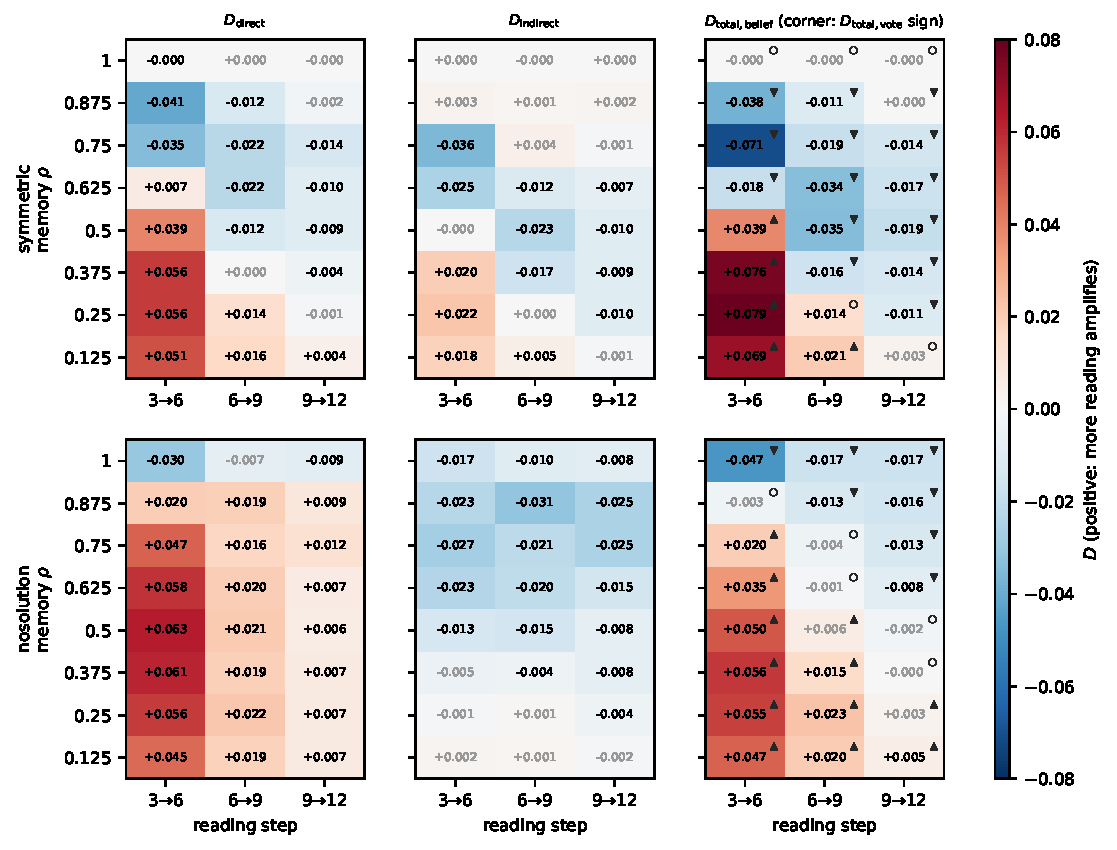
\includegraphics[width=0.98\linewidth]{step2b_fig1_heatmaps.pdf}
\caption{$D_{\rm direct}$, $D_{\rm indirect}$ and $D_{\rm total,belief}$ per reading step and $\rho$; one colour scale
centred on 0; grey number: 95\% interval includes 0. Corner of the right column: sign of $D_{\rm total,vote}$
($\blacktriangle$ positive, $\blacktriangledown$ negative, $\circ$ unresolved).}
\end{figure}

\paragraph{Q1: when does the direct term change sign?}
\begin{itemize}\itemsep1pt
\item \textbf{Symmetric:} $D_{\rm direct}$ turns negative at $\rho = 0.75$ ($3\!\to\!6$), $0.5$ ($6\!\to\!9$) and
  $0.375$ ($9\!\to\!12$): always one $\rho$ value (0.125) \emph{above} the vote boundary ($0.625$, $0.375$, $0.25$). In
  that band the total is already protective while the direct term is still $\ge 0$ (e.g.\ $\rho = 0.625$,
  $3\!\to\!6$: direct $+0.007$, indirect $-0.025$).
\item \textbf{Nosolution:} $D_{\rm direct}$ is positive at every $\rho < 1$ for every step and negative only at
  $\rho = 1$ ($3\!\to\!6$: $-0.030$; $9\!\to\!12$: $-0.009$). It coincides with the vote boundary only for $3\!\to\!6$
  (between 0.875 and 1).
\end{itemize}

\paragraph{Q2: when does the indirect term change sign?}
\begin{itemize}\itemsep1pt
\item \textbf{Nosolution:} never resolved positive. Negative from $\rho = 0.5$ ($3\!\to\!6$), $0.375$ ($6\!\to\!9$),
  $0.25$ ($9\!\to\!12$), largest at $\rho = 0.75$--$0.875$ ($-0.021$ to $-0.031$).
\item \textbf{Symmetric:} positive at low memory ($3\!\to\!6$ at $\rho \le 0.375$: $+0.018$ to $+0.022$; $6\!\to\!9$ at
  $\rho = 0.125$: $+0.005$), negative at intermediate memory (from $\rho = 0.625$, $0.375$, $0.25$ for the three steps, up
  to $\rho = 0.75$), unresolved at $\rho \ge 0.875$, where agents' own facts nearly prove A0 in both arms.
\item \textbf{Meaning, not count:} $D_{\rm indirect}$ hardly follows the change in how many more agent-origin facts the
  silent arm keeps than the controller arm (correlation 0.27 symmetric, $-0.22$ nosolution). It reflects \emph{which}
  original facts are kept, i.e.\ their posterior content.
\end{itemize}

\paragraph{Q3: which mechanism controls each resolved crossover?} Neighbouring resolved cells of opposite sign in each
step column, unresolved cells skipped; classified by $D_{\rm direct}$ on both sides.

\begin{table}[H]
\centering\small
\begin{tabular}{llccl}
\toprule
setup & step & amplifying $\rho$ & protective $\rho$ & mechanism (belief total; vote total gives the same) \\
\midrule
symmetric & $3\!\to\!6$ & 0.5 & 0.625 & indirect override (direct $+0.007$, indirect $-0.025$) \\
symmetric & $6\!\to\!9$ & 0.25 (vote 0.125) & 0.375 & mixed: direct changes sign at the same place (unresolved at 0.375) \\
symmetric & $9\!\to\!12$ & -- & -- & not resolved: no resolved amplifying cell ($\rho = 0.125$ unresolved) \\
nosolution & $3\!\to\!6$ & 0.75 & 1 & direct reversal (direct $+0.047 \to -0.030$; indirect $-0.017$ adds) \\
nosolution & $6\!\to\!9$ & 0.375 (vote 0.5) & 0.875 & indirect override (direct $+0.019$, indirect $-0.031$) \\
nosolution & $9\!\to\!12$ & 0.125 (vote 0.25) & 0.625 & indirect override (direct $+0.007$, indirect $-0.015$) \\
\bottomrule
\end{tabular}
\end{table}

\begin{itemize}\itemsep1pt
\item \textbf{Nosolution:} protection comes from the indirect term overriding a still-positive direct term, except
  at full memory, where the direct term itself reverses.
\item \textbf{Symmetric:} the indirect term tips the total first; the direct term follows one $\rho$ step higher, so
  above the crossover both terms protect (up to $\rho = 0.75$; at $\rho \ge 0.875$ only the direct term).
\item At the belief-level crossover $D_{\rm direct} = -D_{\rm indirect}$ holds by construction; this is an identity at
  zero response, not evidence that the two terms are independent causal pathways.
\end{itemize}

\begin{figure}[H]
\centering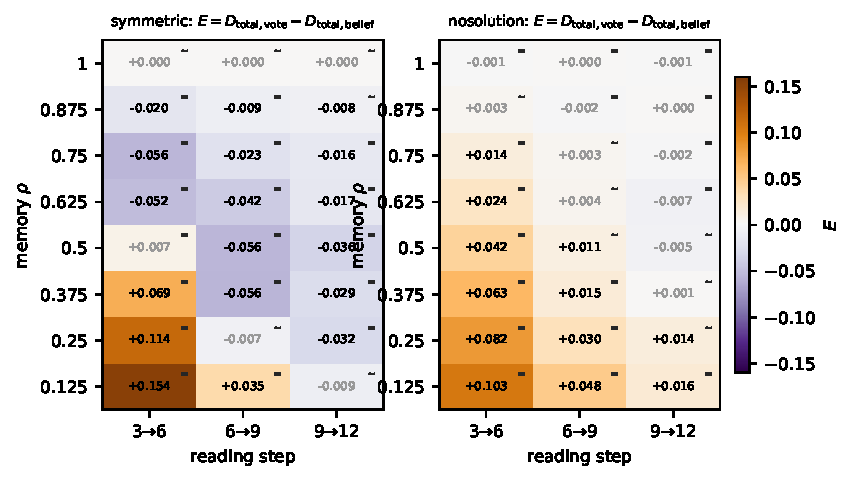
\includegraphics[width=0.75\linewidth]{step2b_fig2_vote_vs_belief.pdf}
\caption{$E = D_{\rm total,vote} - D_{\rm total,belief}$ with 95\% intervals (grey: includes 0). Corner: ``='' when
both totals are resolved with the same sign, ``$\sim$'' when at least one is unresolved (no cell has opposite resolved
signs).}
\end{figure}

\begin{itemize}\itemsep1pt
\item Where both totals are resolved ($\rho < 1$) their signs agree in every cell: 18/18 symmetric, 14/14 nosolution.
\item $E$ is large and systematic, so the two totals differ in size, not in direction.
\end{itemize}

\begin{figure}[H]
\centering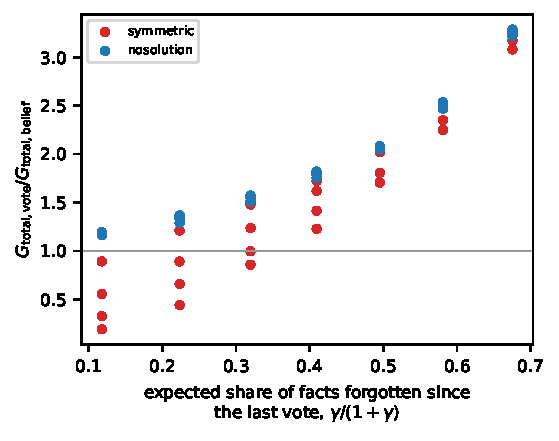
\includegraphics[width=0.42\linewidth]{step2b_fig3_vote_belief_ratio.pdf}
\caption{$G_{\rm total,vote}/G_{\rm total,belief}$ at each $(\rho, q)$ (with $|G_{\rm total,belief}| > 0.02$) against the
expected share of remembered facts forgotten since the agent's last vote, $\gamma/(1+\gamma)$, $\gamma = -\ln\rho$
(agents act at rate 1; observed mean time since the last vote 0.99).}
\end{figure}

\begin{itemize}\itemsep1pt
\item The ratio follows forgetting since the last vote (correlation 0.96 in both setups): votes are 3.2 times the
  snapshot belief shift at $\rho = 0.125$ and 1.5--1.8 times at $\rho = 0.5$. Votes were drawn from fuller memories than
  the $t = 30$ snapshot holds; the snapshot beliefs are compressed toward the prior. Not explained: symmetric
  $\rho = 0.875$, ratio 0.49.
\end{itemize}

\paragraph{Ambiguous cells} (at least one total unresolved, $\rho < 1$; \texttt{tables/step2b\_ambiguous\_cells.csv}).
Symmetric: $(0.25, 6\!\to\!9)$ belief $+$, vote unresolved; $(0.125, 9\!\to\!12)$ both unresolved; $(0.875,
9\!\to\!12)$ vote $-$, belief unresolved. Nosolution: $(0.875, 3\!\to\!6)$, $(0.625, 6\!\to\!9)$, $(0.75, 6\!\to\!9)$,
$(0.375, 9\!\to\!12)$, $(0.5, 9\!\to\!12)$ both unresolved; $(0.5, 6\!\to\!9)$ and $(0.25, 9\!\to\!12)$ vote $+$,
belief unresolved. All lie on or next to the crossovers.

\paragraph{Limitations.} Beliefs are taken from the memory snapshot at $t = 30$; votes were cast at each agent's last
activation, from the memory it held then. The run did not record per-action memories, so the belief at the last vote
cannot be recovered exactly (between that action and $t = 30$ an agent only loses facts, and which ones is not
stored). As agreed, this is reported, not resolved. It affects magnitudes (Figure 3), not the signs where both are
resolved. One world per setup, $N = 24$.

\paragraph{Audit: are further runs needed for this question?} No.
\begin{itemize}\itemsep1pt
\item $q_c$, $\lambda_c$, $B$, $W$: those runs have no memory records, so they cannot be decomposed. Their vote-level
  reversal signs agree with the main setting across all 72 $q_c \times$ rate $\times$ gate combinations and all three
  variants (step 1). Not needed.
\item More $(\rho, q)$: the crossovers are bracketed to one $\rho$ step (0.125) in every column except symmetric
  $9\!\to\!12$, whose amplifying side would need $\rho < 0.125$.
\item Smallest useful run, only if exact magnitudes matter: the same 128 settings re-run with per-action records
  (same seed, identical trajectories; about 10 minutes, about 6 GB) to evaluate beliefs at the last vote.
\end{itemize}

\paragraph{Files.} Script \texttt{scripts/s2b\_decomposition.py} and \texttt{scripts/s2b\_figures.py}; tables
\texttt{tables/step2b\_D.csv} (every $D$ and $E$ with intervals and signs), \texttt{step2b\_G.csv},
\texttt{step2b\_reversals.csv}, \texttt{step2b\_checks.csv}, \texttt{step2b\_vote\_age.csv},
\texttt{step2b\_validation.csv}; episode values \texttt{results/key\_phenomena/s2b\_episodes.parquet}.

\end{document}
